\documentclass[a4paper,12pt]{article}

\usepackage{hyperref}
\usepackage{graphicx}

\hypersetup{
  pdftitle={Flying Fist},
  pdfauthor={Kimmo Puputti, Morocz Adam},
  pdfsubject={},
  pdfcreator={},
  pdfproducer={pdflatex},
  pdfkeywords={},
  colorlinks=true,
  linkcolor=red,
  citecolor=green,
  filecolor=magenta,
  urlcolor=blue
}

\title{Web Technology 2II25:\\Flying Fist - final report}
\author{Kimmo Puputti, kimmo.puputti@tkk.fi, 0735552\\M\'orocz \'Ad\'am, morocz@gmail.com, }

\begin{document}

\maketitle

\section{Introduction}

Everything that people do is somehow related to geographical
information. This is why a lot of the resources in WWW contain
geographical information. Place names, however, can be very ambiguous
and it can be hard to distinguish places from text
content. Geographical data is very linked within itself and
geographically annotated data can be easily linked together.

Our application lets you browse geographical data that is linked
within itself and also to other third party sites like Wikipedia
etc. We use the data from
Geonames\footnote{\url{http://www.geonames.org/}} for places inside
The Netherlands in the backend of our application.

You can search for places by their name and browse through the pages
of each place. Every place is linked to several other places. You can
also see the places on an interactive map.

\section{Data and the ontology}

The feature data downloaded from the Geonames site was converted into
an RDF graph and serialized into the N3 format. The ontology has 675
classes, 15 properties, and 21 372 feature instances, totaling in over
300 000 RDF triples.

Creating the ontology was straight-forward. All the feature type
classes formed a clear hierarchy and the properties were constructed
from the data schema. The flexibility of the RDF format really helped
in that we didn't have to fix the schema and it was trivial to add new
properties and to list all properties in the resource's page.

The data was very linked within itself, but also to other resources on
the web. We combined it with weather information and Wikipedia pages
using the Geonames API, but there is no limits in what could be added
to enrich the application. For example, images and news could be shown
for each place.

\section{Tool and Technologies}

\subsection{Backend}

The web application is built in Python using CherryPy HTTP framework
and Mako templates. The data is converted into RDF and queried using
RDFLib. The triple store is read into memory from the converted N3
files every time the application is started. We also use
PyLucene\footnote{\url{http://lucene.apache.org/pylucene/}} to index
and search the place names.

\subsection{Frontend}

The HTML is built using Mako templates. We use jQuery JavaScript
library\footnote{\url{http://jquery.com/}} for the dynamic frontend
functionality and AJAX calls and Google Maps JavaScript API
V3\footnote{\url{http://code.google.com/apis/maps/documentation/javascript/}}
for the interactive map.

The layout of the application is done using CSS.

\section{Using the application}

\subsection{Setup}

\noindent \textit{Prerequisites}: CherryPy, Mako, PyLucene, RDFLib,
and RDF Extras (from RDFLib) have to be installed and found on the
Python search path.\\

\noindent To run the application, the Git repository has to be cloned
first with the following command:

\begin{verbatim}
git clone git://github.com/kpuputti/webtech.git
\end{verbatim}

\noindent which creates a directory `webtech' that has the `project'
subdirectory with all the source code.

Second, some directories have to be made into the project directory
using the command:

\begin{verbatim}
mkdir data index log output
\end{verbatim}

\noindent Third, the following files must be downloaded from the
Geonames download
server\footnote{\url{http://download.geonames.org/export/dump/}} and
extracted into the `data' directory:

\begin{verbatim}
NL.zip
admin1Codes.txt
admin2Codes.txt
countryInfo.txt
featureCodes_en.txt
\end{verbatim}

\noindent Then using the control script \texttt{fist.py} in the
project root folder, the RDF triple store and the Lucene index are
created with the commands:

\begin{verbatim}
python fist.py create_storage
python fist.py create_index
\end{verbatim}

\noindent The RDF graphs are stored in the `output' directory and the
Lucene index in the `index' directory. The log file for the
application is created in the `log' directory and can be followed to
get information of the progress or about errors that might have
happened.

If the backend storages are created successfully, the application can
be started with the command:

\begin{verbatim}
python fist.py run
\end{verbatim}

\subsection{User Interface}

All the features in the triple store have their own page. A map is
showing where the feature is and the features properties are listed
under the map. Also the current weather conditions are fetched
dynamically from the Geonames API.

As seen in Figure \ref{feature}, Wikipedia pages are also shown on the
map nearby the current place if the checkbox is checked. The data is
fetched dynamically as an AJAX call to the internal REST-style JSON
API that fetches the information from the Geonames API.

\begin{figure}[h]
  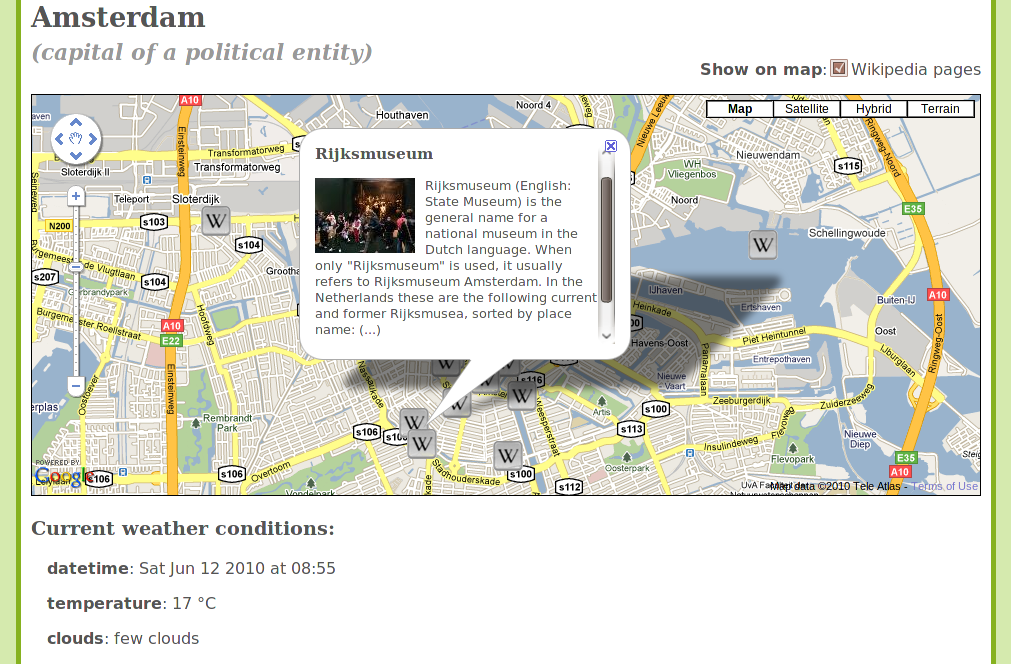
\includegraphics[width=\linewidth]{img/feature.png}
  \caption{Wikipedia pages and weather conditions near the place.}
  \label{feature}
\end{figure}

The same feature page is used for all browsable RDF resources. The
data is highly linked and can therefore be easily browsed following
the internal or external links. On the bottom of each resource's page,
a list of recommended places is shown. Also the property name that
links these two resources is shown in the recommendations (Figure
\ref{recommendations}).

\begin{figure}[h]
  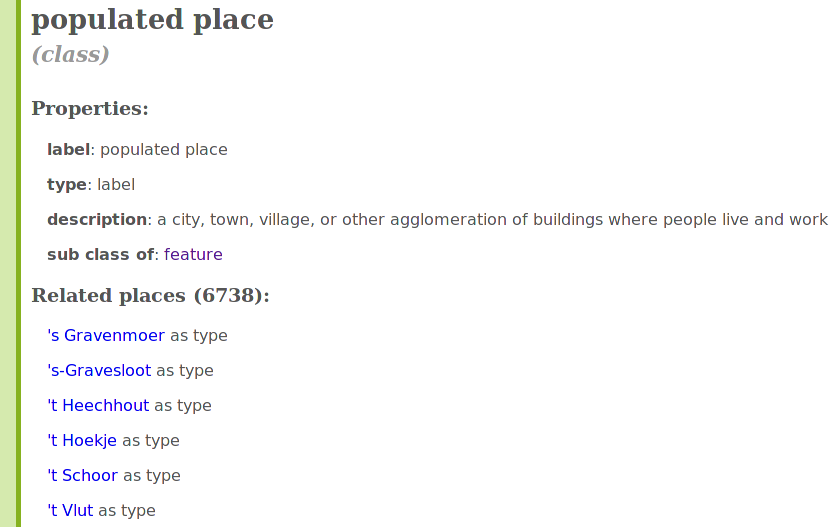
\includegraphics[width=\linewidth]{img/recommendations.png}
  \caption{Properties and a list of related resources are shown.}
  \label{recommendations}
\end{figure}

\noindent The search has an autocomplete feature that suggests place
names based on what the user is writing into the search box (Figure
\ref{autocomplete}). Matched tokens are highlighted. The autocomplete
feature is especially useful for slow typists or when searching long
place names.

\begin{figure}[h]
  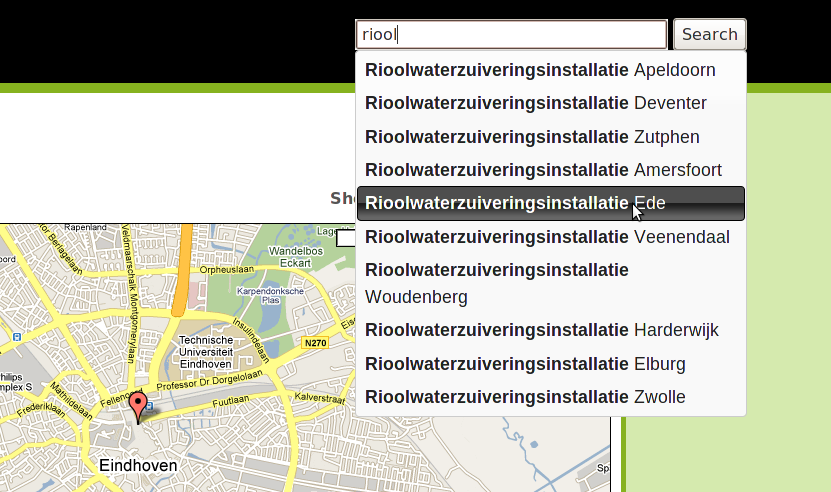
\includegraphics[width=\linewidth]{img/autocomplete.png}
  \caption{Autocomplete search suggests place names.}
  \label{autocomplete}
\end{figure}

The search results page (Figure \ref{search}) lists places whose name
matches the search query. The results are listed in an order where the
best match is first. Place type, its admin codes (area where the place
is), and population are shown for each result (if found). Also, a
small map image is shown for the best result.

\begin{figure}[h]
  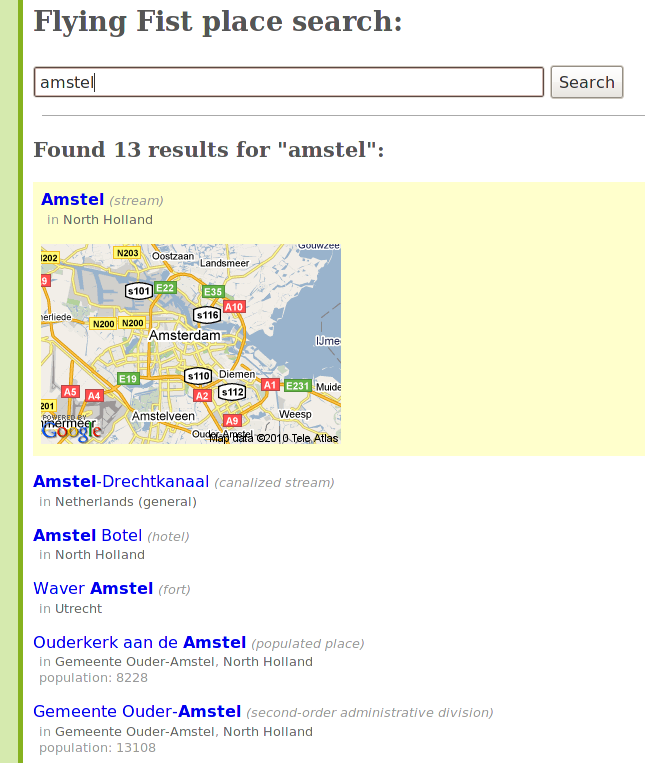
\includegraphics[width=\linewidth]{img/search.png}
  \caption{Results for the query `amstel'.}
  \label{search}
\end{figure}

\clearpage
\section{Conclusions}

We created a web application to browse geographical data that is
highly linked within itself as well as with other resources in the
web. The backend data store uses RDF to present the data using
triples. The use of RDF provided a flexible format that can be used
for changing or heterogeneous data.

The search feature of our application got a lot of attention and we
are very pleased with the results. The use of the search is easy and
intuitive, and the provided results are relevant with respect to the
query.

The browsing of the places is easy and a lot of information is
provided for each resource. The browsing was also made as general as
possible, so that it could not only be used for places, but for all
resources in the ontology. Using RDF in the backend really made this
possible. It as also nice to add external information to enrich the
data.

\end{document}
